\documentclass[reqno]{amsbook}
\usepackage[utf8]{inputenc}
\usepackage{HBSuerDemir}
\usepackage{subcaption}
\usepackage{caption}

\begin{document}

    \hPage{b1p2/316}
    \noindent-r, the limaçon has then the equation
    \begin{equation}
        r = a + \delta cos \theta \tag{1^{\prime\prime}}
    \end{equation}
    \noindent where $\hAbs{a}$ = $\ell$.\\
    \indent Rotating the limaçon about the pole by the angles $\pi/2$, $\pi$, $3\pi/2$ we have the following equations:
    \[
        r =  a + \delta sin \theta,\quad r = a - \delta cos \theta,\quad r = a - \delta sin \theta
    \]
    Hence an equation of the form
    \[
        r = a + b_{1} cos \theta\quad \textrm{or}\quad r = a + b_{1} sin \theta
    \]
    represents a limaçon of PASCAL with $\ell$ = $\hAbs{a}$ and $\delta$ = $b_{1}$.\\
    \indent Now rotating the PA, by an angle $a$, the equation
    \[
        r=a+ b_{1} cos(\theta-\alpha) \quad \textrm{or}\quad r=a + b_{1} sin(\theta-\alpha)
    \]
    is obtained which is in the form (primes being dropped):
    \begin{equation}
        r = a + b cos \theta + c sin \theta \tag{2}
    \end{equation}
    where $\ell$ = $\hAbs{a}$ and $\delta$ = $\sqrt{b^2 + c^2}$.\\
    \indent A limaçon can be treated continuously as follows: Drawing a circle and marking on a ruler three points $P'$, $M$, $P$ such that $\hAbs{P'M}$=$\hAbs{MP}$, and moving the ruler in such a way that it always passes through fixed point 0 of the circle and $M$ lying always on the circle (do it!)\\
    \indent For various values of $\delta$ and $\ell$, limaçons appear to be of three types shown below: 
    
    \begin{figure}[h]
      \centering
      \begin{minipage}{0.3\textwidth}
        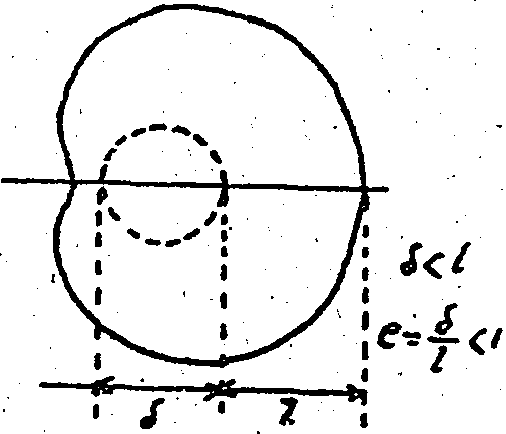
\includegraphics[width=\textwidth]{images/b1p2-316-fig01.png}
        \caption*{Elliptic case}
      \end{minipage}
      \begin{minipage}{0.3\textwidth}
        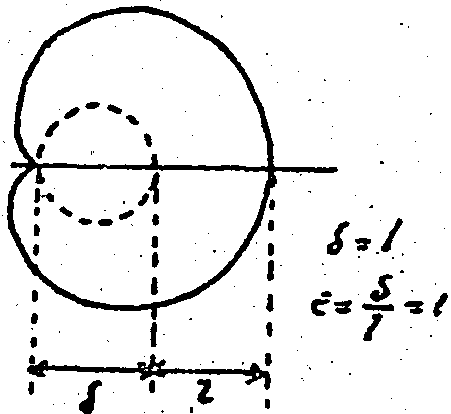
\includegraphics[width=\textwidth]{images/b1p2-316-fig02.png}
        \caption*{\parbox{\textwidth}{Parabolic case\\ (a cardioid)}}
      \end{minipage}
      \begin{minipage}{0.3\textwidth}
        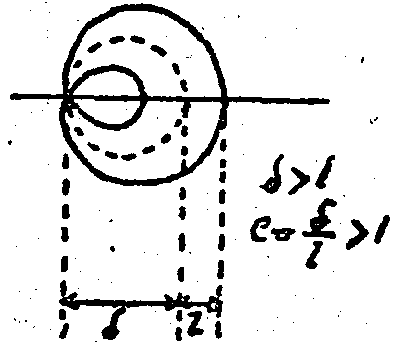
\includegraphics[width=\textwidth]{images/b1p2-316-fig03.png}
        \caption*{Hyperbolic case}
      \end{minipage}
    \end{figure}

\end{document}
